\documentclass[final,3p,twocolumn]{elsarticle}

\usepackage{amssymb}
\usepackage{mathtools}
\usepackage{tikz}
\usepackage{pgfplots}

\biboptions{super, square, sort&compress}

\pgfplotsset{width=\columnwidth, height=0.6\columnwidth, compat=1.8}
\usepgfplotslibrary{groupplots, external}
\tikzexternalize

\journal{MPhil in Scientific Computing}

\begin{document}

\begin{frontmatter}

\title{Multimaterial Simulations using the Ghost Fluid Method}

\author{Knut Sverdrup}

\address{Cavendish Laboratory, Department of Physics, J J Thomson
  Avenue, Cambridge. CB3 0HE}

\begin{abstract}
    The unsteady, compressible Euler equations for multimaterial flow in one
    dimension have been solved numerically by employing a level set method and
    two versions of the Ghost Fluid Method. 
\end{abstract}

\end{frontmatter}

\section{Introduction}
\label{sec:introduction}

\emph{Literature review. Write about the usefulness of solving Euler eqs and
    CFD in general.  What has happened historiccaly in the understanding of
    these? Different solvers, especially considerations of multi-material cases
    and use of level set methods. }

The Euler equations govern adiabatic and inviscid flow of a fluid. In one
dimension, with density $\rho$, velocity $u$, total energy $E$ and pressure
$p$, they are given by 

\begin{equation}
    \frac{\partial {\bf U}}{\partial t} 
    + \frac{\partial {\bf F(U)}}{\partial x} = 0\,,
    \label{eq:euler}
\end{equation}
%
where the vectors of conserved quantities ${\bf U}$ and their fluxes ${\bf F(U)}$ are given by

\begin{equation*}
    {\bf U} = 
    \begin{bmatrix} 
        \rho \\ 
        \rho u \\ 
        E 
    \end{bmatrix}
    \,,\quad
    {\bf F} = 
    \begin{bmatrix}
        \rho u \\ 
        \rho u^2 + p \\
        u(E+p) 
    \end{bmatrix}
    \,.
\end{equation*}
%
It is sometimes convenient to work in terms of the primitive variables ${\bf W} =
\begin{pmatrix} \rho, & u, & p \end{pmatrix}^T$. The total energy is the sum of
the kinetic and potential energy of the system, i.e.~ 

\begin{equation}
    E = \frac{1}{2} \rho u^2 + \rho e \,,
    \label{eq:energy}
\end{equation}
%
where $e$ is the internal energy, related to the other variables through the
equation of state. For an ideal gas, the equation of state is 

\begin{equation}
     e = \frac{p}{(\gamma-1)\rho} \,,
     \label{eq:EoS}
 \end{equation}
%
where $\gamma$ denotes the ratio of specific heats for the gas. Several other
fluids can be approximated by a so-called stiffened ideal gas equation of
state, 

\begin{equation}
    e = \frac{p+\gamma p_{\infty}}{(\gamma-1)\rho} \,.
    \label{eq:stiffEoS}
\end{equation}
%
Here, a material-dependent stiffening parameter $p_{\infty}$ has been
introduced. Note that Eq. \eqref{eq:stiffEoS} reduces to Eq. \eqref{eq:EoS} for
materials with $p_{\infty}=0$. 

\emph{Which special considerations need to be taken into account for
multimaterial flow? Differences in EoS means we need to think carefully about
material interfaces.}

The numerical methods which have been employed are explained in section
\ref{sec:numerical}, before several test cases and their results are discussed
in section \ref{sec:results}. Section \ref{sec:conclusion} concludes the
report.

\section{Numerical methods}
\label{sec:numerical}

\subsection{Numerical solutions for the Riemann Problem}
\label{subsec:riemann}

Given a conservation equation and two sets of piecewise constant states
separated by a single discontinuity, the initial value problem of evolving this
system in time is called a Riemann problem. It is very useful in the study of
the Euler equations for two reasons. Firstly, it allows for exact (up to an
arbitrary accuracy) solutions for systems obeying Eq.  \eqref{eq:euler} which
have a single contact discontinuity. Secondly, the discretization of space
which is inevitable in computational schemes for solving differential
equations, allows for precise solvers of conservation equations based on the
solutions of many local Riemann problems. 

For the Euler equations and initial conditions 

\begin{equation*}
    {\bf W}(x,t=0) = 
    \begin{cases}
        {\bf W}_L, \,&x \leq 0 \\ 
        {\bf W}_R, \,&x > 0 \\ 
    \end{cases} \,,
\end{equation*}
%
Figure \ref{fig:riemann} shows typical states the system can have, in addition
to characteristics for waves propagating in space-time. There are two types of
resultant waves that propagate through space, in addition to the contact wave
(dashed). The first is a shock wave, depicted as a thick line on the left,
while the second is a rarefaction wave, shown as several gradually decaying (in
strength) lines on the left. Any combination of shock and rarefaction waves can
occur on the left and right sides of the contact discontinuity, and the result
is only dependent on ${\bf W}(x,0)$. 

\begin{figure}[htb]
    \centering
    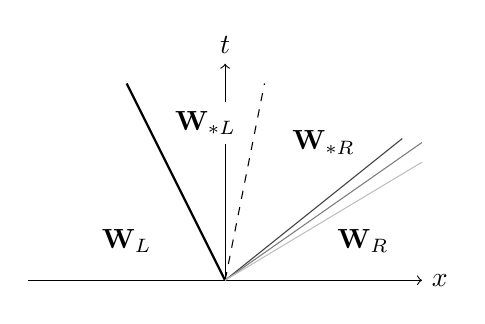
\begin{tikzpicture}[scale=2.5]
        \coordinate (origin) at (0,0);
        \coordinate (left) at (-1,0);
        \coordinate (right) at (1,0);
        \coordinate (top) at (0,1.1);
        \draw[->] (left) -- (right) node[right]{$x$};
        \draw[->] (origin) -- (top) node[above]{$t$};
        \draw[thick] (origin) -- (-0.5,1) {};
        \draw[dashed] (origin) -- (0.2,1) {};
        \draw[black!75] (origin) -- (0.9,0.72) {};
        \draw[black!50] (origin) -- (1,0.7) {};
        \draw[black!25] (origin) -- (1,0.6) {};
        \node () at (-0.5,0.2) {${\bf W}_L$};
        \node[fill=white] () at (-0.1,0.8) {${\bf W}_{*L}$};
        \node () at (0.5,0.7) {${\bf W}_{*R}$};
        \node () at (0.7,0.2) {${\bf W}_R$};
    \end{tikzpicture}
    \caption{Possible wave configurations for the Riemann problem for Euler's
    equations in one dimension.}
    \label{fig:riemann}
\end{figure}

\emph{History of solving Riemann problems. Mention different approximate
solvers.}

\emph{For this project, the exact solver has been implemented.}

\emph{Each of the four states separated by the waves are constant.
Additionally, pressure and velocity is constant for the star states. How much
more should be said about this? }

\subsection{Schemes for the Euler equations}
\label{subsec:eulerschemes}

Explain the order of schemes and the difference between centered and RP-based
schemes. 

\subsubsection{Slope-Limiting Centered (SLIC)}
\label{subsubsec:slic}

\subsubsection{Weighted-Average Flux (WAF)}
\label{subsubsec:waf}

\subsection{Level-set method}
\label{subsec:levelset}

\subsection{Ghost Fluid Methods}
\label{subsec:ghostfluid}

\subsubsection{Original Ghost Fluid Method}
\label{subsubsec:ogfm}

\subsubsection{Riemann Ghost Fluid Method}
\label{subsubsec:rgfm}

\section{Results}
\label{sec:results}

\subsection{Moving contact discontinuity}
\label{subsec:moving}

\subsection{Simple ghost fluid tests}
\label{subsec:toro}

\subsection{Multimaterial shock tubes for gases}
\label{subsec:shocktubes}

\pgfplotstableread{../Results/testC_OGFM_N100.out}{\one}
\pgfplotstableread{../Results/testC_OGFM_N200.out}{\two}
\pgfplotstableread{../Results/testC_OGFM_N400.out}{\four}

\begin{figure*}[htb]
    \centering
    \begin{tikzpicture}
        \begin{groupplot}[
            group style={group size=2 by 2}, 
            xlabel=$x$, xmin=0, xmax=1, 
            ylabel style={rotate=-90}]

            \nextgroupplot[ylabel=$\rho$]
            \addplot+[only marks, mark=triangle, color=teal, each nth point=1]
            table[x={x}, y={rho}]{\one};
            \addplot+[only marks, mark=x, color=red, each nth point=2]
            table[x={x}, y={rho}]{\two};
            \addplot+[only marks, mark=o, color=blue,  mark size=1pt, each nth point=4]
            table[x={x}, y={rho}]{\four};

            \nextgroupplot[ylabel=$u$, ytick pos=right]
            \addplot+[only marks, mark=triangle, color=teal, each nth point=1]
            table[x={x}, y={u}]{\one};
            \addplot+[only marks, mark=x, color=red, each nth point=2]
            table[x={x}, y={u}]{\two};
            \addplot+[only marks, mark=o, color=blue,  mark size=1pt, each nth point=4]
            table[x={x}, y={u}]{\four};

            \nextgroupplot[ylabel=$p$]
            \addplot+[only marks, mark=triangle, color=teal, each nth point=1]
            table[x={x}, y={p}]{\one};
            \addplot+[only marks, mark=x, color=red, each nth point=2]
            table[x={x}, y={p}]{\two};
            \addplot+[only marks, mark=o, color=blue,  mark size=1pt, each nth point=4]
            table[x={x}, y={p}]{\four};

            \nextgroupplot[ylabel=$e$, ytick pos=right]
            \addplot+[only marks, mark=triangle, color=teal, each nth point=1]
            table[x={x}, y={e}]{\one};
            \addplot+[only marks, mark=x, color=red, each nth point=2]
            table[x={x}, y={e}]{\two};
            \addplot+[only marks, mark=o, color=blue,  mark size=1pt, each nth point=4]
            table[x={x}, y={e}]{\four};

        \end{groupplot}
    \end{tikzpicture}
\caption{Original Ghost Fluid method for test C.
    \textcolor{teal}{$\triangle$}$N=100$
    \textcolor{red}{$\times$}$N=200$
    \textcolor{blue}{$\circ$}$N=400$ }
\label{fig:testC_OGFM}
\end{figure*}

\pgfplotstableread{../Results/testC_RGFM_N100.out}{\one}
\pgfplotstableread{../Results/testC_RGFM_N200.out}{\two}
\pgfplotstableread{../Results/testC_RGFM_N400.out}{\four}

\begin{figure*}[htb]
    \centering
    \begin{tikzpicture}
        \begin{groupplot}[
            group style={group size=2 by 2}, 
            xlabel=$x$, xmin=0, xmax=1, 
            ylabel style={rotate=-90}]

            \nextgroupplot[ylabel=$\rho$]
            \addplot+[only marks, mark=triangle, color=teal, each nth point=1]
            table[x={x}, y={rho}]{\one};
            \addplot+[only marks, mark=x, color=red, each nth point=2]
            table[x={x}, y={rho}]{\two};
            \addplot+[only marks, mark=o, color=blue,  mark size=1pt, each nth point=4]
            table[x={x}, y={rho}]{\four};

            \nextgroupplot[ylabel=$u$, ytick pos=right]
            \addplot+[only marks, mark=triangle, color=teal, each nth point=1]
            table[x={x}, y={u}]{\one};
            \addplot+[only marks, mark=x, color=red, each nth point=2]
            table[x={x}, y={u}]{\two};
            \addplot+[only marks, mark=o, color=blue,  mark size=1pt, each nth point=4]
            table[x={x}, y={u}]{\four};

            \nextgroupplot[ylabel=$p$]
            \addplot+[only marks, mark=triangle, color=teal, each nth point=1]
            table[x={x}, y={p}]{\one};
            \addplot+[only marks, mark=x, color=red, each nth point=2]
            table[x={x}, y={p}]{\two};
            \addplot+[only marks, mark=o, color=blue,  mark size=1pt, each nth point=4]
            table[x={x}, y={p}]{\four};

            \nextgroupplot[ylabel=$e$, ytick pos=right]
            \addplot+[only marks, mark=triangle, color=teal, each nth point=1]
            table[x={x}, y={e}]{\one};
            \addplot+[only marks, mark=x, color=red, each nth point=2]
            table[x={x}, y={e}]{\two};
            \addplot+[only marks, mark=o, color=blue,  mark size=1pt, each nth point=4]
            table[x={x}, y={e}]{\four};

        \end{groupplot}
    \end{tikzpicture}
\caption{Riemann Ghost Fluid method for test C.
    \textcolor{teal}{$\triangle$}$N=100$
    \textcolor{red}{$\times$}$N=200$
    \textcolor{blue}{$\circ$}$N=400$ }
\label{fig:testC_RGFM}
\end{figure*}

\pgfplotstableread{../Results/testD_OGFM_N100.out}{\one}
\pgfplotstableread{../Results/testD_OGFM_N200.out}{\two}
\pgfplotstableread{../Results/testD_OGFM_N400.out}{\four}

\begin{figure*}[htb]
    \centering
    \begin{tikzpicture}
        \begin{groupplot}[
            group style={group size=2 by 2}, 
            xlabel=$x$, xmin=0, xmax=1, 
            ylabel style={rotate=-90}]

            \nextgroupplot[ylabel=$\rho$]
            \addplot+[only marks, mark=triangle, color=teal, each nth point=1]
            table[x={x}, y={rho}]{\one};
            \addplot+[only marks, mark=x, color=red, each nth point=2]
            table[x={x}, y={rho}]{\two};
            \addplot+[only marks, mark=o, color=blue,  mark size=1pt, each nth point=4]
            table[x={x}, y={rho}]{\four};

            \nextgroupplot[ylabel=$u$, ytick pos=right]
            \addplot+[only marks, mark=triangle, color=teal, each nth point=1]
            table[x={x}, y={u}]{\one};
            \addplot+[only marks, mark=x, color=red, each nth point=2]
            table[x={x}, y={u}]{\two};
            \addplot+[only marks, mark=o, color=blue,  mark size=1pt, each nth point=4]
            table[x={x}, y={u}]{\four};

            \nextgroupplot[ylabel=$p$]
            \addplot+[only marks, mark=triangle, color=teal, each nth point=1]
            table[x={x}, y={p}]{\one};
            \addplot+[only marks, mark=x, color=red, each nth point=2]
            table[x={x}, y={p}]{\two};
            \addplot+[only marks, mark=o, color=blue,  mark size=1pt, each nth point=4]
            table[x={x}, y={p}]{\four};

            \nextgroupplot[ylabel=$e$, ytick pos=right]
            \addplot+[only marks, mark=triangle, color=teal, each nth point=1]
            table[x={x}, y={e}]{\one};
            \addplot+[only marks, mark=x, color=red, each nth point=2]
            table[x={x}, y={e}]{\two};
            \addplot+[only marks, mark=o, color=blue,  mark size=1pt, each nth point=4]
            table[x={x}, y={e}]{\four};

        \end{groupplot}
    \end{tikzpicture}
\caption{Original Ghost Fluid method for test D. 
    \textcolor{teal}{$\triangle$}$N=100$
    \textcolor{red}{$\times$}$N=200$
    \textcolor{blue}{$\circ$}$N=400$ }
\label{fig:testD_OGFM}
\end{figure*}

\pgfplotstableread{../Results/testD_RGFM_N100.out}{\one}
\pgfplotstableread{../Results/testD_RGFM_N200.out}{\two}
\pgfplotstableread{../Results/testD_RGFM_N400.out}{\four}

\begin{figure*}[htb]
    \centering
    \begin{tikzpicture}
        \begin{groupplot}[
            group style={group size=2 by 2}, 
            xlabel=$x$, xmin=0, xmax=1, 
            ylabel style={rotate=-90}]

            \nextgroupplot[ylabel=$\rho$]
            \addplot+[only marks, mark=triangle, color=teal, each nth point=1]
            table[x={x}, y={rho}]{\one};
            \addplot+[only marks, mark=x, color=red, each nth point=2]
            table[x={x}, y={rho}]{\two};
            \addplot+[only marks, mark=o, color=blue,  mark size=1pt, each nth point=4]
            table[x={x}, y={rho}]{\four};

            \nextgroupplot[ylabel=$u$, ytick pos=right]
            \addplot+[only marks, mark=triangle, color=teal, each nth point=1]
            table[x={x}, y={u}]{\one};
            \addplot+[only marks, mark=x, color=red, each nth point=2]
            table[x={x}, y={u}]{\two};
            \addplot+[only marks, mark=o, color=blue,  mark size=1pt, each nth point=4]
            table[x={x}, y={u}]{\four};

            \nextgroupplot[ylabel=$p$]
            \addplot+[only marks, mark=triangle, color=teal, each nth point=1]
            table[x={x}, y={p}]{\one};
            \addplot+[only marks, mark=x, color=red, each nth point=2]
            table[x={x}, y={p}]{\two};
            \addplot+[only marks, mark=o, color=blue,  mark size=1pt, each nth point=4]
            table[x={x}, y={p}]{\four};

            \nextgroupplot[ylabel=$e$, ytick pos=right]
            \addplot+[only marks, mark=triangle, color=teal, each nth point=1]
            table[x={x}, y={e}]{\one};
            \addplot+[only marks, mark=x, color=red, each nth point=2]
            table[x={x}, y={e}]{\two};
            \addplot+[only marks, mark=o, color=blue,  mark size=1pt, each nth point=4]
            table[x={x}, y={e}]{\four};

        \end{groupplot}
    \end{tikzpicture}
\caption{Riemann Ghost Fluid method for test D. 
    \textcolor{teal}{$\triangle$}$N=100$
    \textcolor{red}{$\times$}$N=200$
    \textcolor{blue}{$\circ$}$N=400$ }
\label{fig:testD_RGFM}
\end{figure*}
\subsection{Water-gas shock tube test}
\label{subsec:water}

\pgfplotstableread{../Results/testE_RGFM_N100.out}{\one}
\pgfplotstableread{../Results/testE_RGFM_N200.out}{\two}
\pgfplotstableread{../Results/testE_RGFM_N400.out}{\four}
\pgfplotstableread{../Results/testE_RGFM_N1000.out}{\tausen}

\begin{figure*}[htb]
    \centering
    \begin{tikzpicture}
        \begin{groupplot}[
            group style={group size=2 by 2}, 
            xlabel=$x$, xmin=0, xmax=1, 
            ylabel style={rotate=-90}]

            \nextgroupplot[ylabel=$\rho$]
            \addplot+[mark=none, color=black]
            table[x={x}, y={rhoEx}]{\tausen};
            \addplot+[only marks, mark=triangle, color=teal, each nth point=1]
            table[x={x}, y={rho}]{\one};
            \addplot+[only marks, mark=x, color=red, each nth point=2]
            table[x={x}, y={rho}]{\two};
            \addplot+[only marks, mark=o, color=blue,  mark size=1pt, each nth point=4]
            table[x={x}, y={rho}]{\four};

            \nextgroupplot[ylabel=$u$, ytick pos=right]
            \addplot+[mark=none, color=black]
            table[x={x}, y={uEx}]{\tausen};
            \addplot+[only marks, mark=triangle, color=teal, each nth point=1]
            table[x={x}, y={u}]{\one};
            \addplot+[only marks, mark=x, color=red, each nth point=2]
            table[x={x}, y={u}]{\two};
            \addplot+[only marks, mark=o, color=blue,  mark size=1pt, each nth point=4]
            table[x={x}, y={u}]{\four};

            \nextgroupplot[ylabel=$p$]
            \addplot+[mark=none, color=black]
            table[x={x}, y={pEx}]{\tausen};
            \addplot+[only marks, mark=triangle, color=teal, each nth point=1]
            table[x={x}, y={p}]{\one};
            \addplot+[only marks, mark=x, color=red, each nth point=2]
            table[x={x}, y={p}]{\two};
            \addplot+[only marks, mark=o, color=blue,  mark size=1pt, each nth point=4]
            table[x={x}, y={p}]{\four};

            \nextgroupplot[ylabel=$e$, ytick pos=right]
            \addplot+[mark=none, color=black]
            table[x={x}, y={eEx}]{\tausen};
            \addplot+[only marks, mark=triangle, color=teal, each nth point=1]
            table[x={x}, y={e}]{\one};
            \addplot+[only marks, mark=x, color=red, each nth point=2]
            table[x={x}, y={e}]{\two};
            \addplot+[only marks, mark=o, color=blue,  mark size=1pt, each nth point=4]
            table[x={x}, y={e}]{\four};

        \end{groupplot}
    \end{tikzpicture}
    \caption{Riemann Ghost Fluid method for test E.
    \textcolor{teal}{$\triangle$}$N=100$
    \textcolor{red}{$\times$}$N=200$
    \textcolor{blue}{$\circ$}$N=400$ }
\label{fig:testE_RGFM}
\end{figure*}

\begin{figure*}[htb]
    \centering
    \begin{tikzpicture}
        \begin{groupplot}[
            group style={group size=2 by 2}, 
            xlabel=$x$, xmin=0, xmax=1, 
            ylabel style={rotate=-90}]

            \nextgroupplot[ylabel=$\rho$]
            \addplot+[mark=none, color=black]
            table[x={x}, y={rhoEx}]{\tausen};
            \addplot+[only marks, mark=o, color=blue,  mark size=1pt, each nth point=10]
            table[x={x}, y={rho}]{\tausen};

            \nextgroupplot[ylabel=$u$, ytick pos=right]
            \addplot+[mark=none, color=black]
            table[x={x}, y={uEx}]{\tausen};
            \addplot+[only marks, mark=o, color=blue,  mark size=1pt, each nth point=10]
            table[x={x}, y={u}]{\tausen};

            \nextgroupplot[ylabel=$p$]
            \addplot+[mark=none, color=black]
            table[x={x}, y={pEx}]{\tausen};
            \addplot+[only marks, mark=o, color=blue,  mark size=1pt, each nth point=10]
            table[x={x}, y={p}]{\tausen};

            \nextgroupplot[ylabel=$e$, ytick pos=right]
            \addplot+[mark=none, color=black]
            table[x={x}, y={eEx}]{\tausen};
            \addplot+[only marks, mark=o, color=blue,  mark size=1pt, each nth point=10]
            table[x={x}, y={e}]{\tausen};

        \end{groupplot}
    \end{tikzpicture}
\caption{Riemann Ghost Fluid method for test E with higher accuracy ($N=1000$).}
\label{fig:testE_RGFM_N1000}
\end{figure*}
\section{Conclusions}
\label{sec:conclusion}

\bibliographystyle{elsarticle-num}
\bibliography{references.bib}


\section*{Acknowledgements}
\label{sec:acknowledgements}
Thanks Steve. 

\end{document}
